\phaseportada{PHASE 5}{Supervised Imitation Learning}{
    % Tech Stack
    XGBoost, Naive Bayes, Logistic Regression, SHAP (Shapley Additive exPlanations), Mutual Information (MI), Chi-Squared ($\chi^2$), Stratified K-Fold CV.
}{
    % Core Challenge
    Overcoming the "Gravitational Well" of highly imbalanced data, where deterministic majority-class noise (obvious rejections) cannibalizes the machine's ability to learn nuanced, high-level strategy.
}{
    % Key Insight
    The agent's decision-making is hierarchical, not flat. By deploying a "Cognitive Cascade" that triages basic logistical failures first, a secondary model can dedicate its full capacity to mapping complex behavioral mechanics like the Sunk Cost Effect and Income Targeting.
}{
    % Operational Outcome
    The successful deployment of a hierarchical XGBoost clone that matched the human agent's strategic efficiency while capturing a 5.7\% volume surplus by eliminating cognitive fatigue.
}

\section{Phase 5 - Supervised Imitation Learning: From Sky to Psyche}


\noindent \textbf{Timeline: January 3 -- January 12, 2026}

The objective of Phase 5 was to synthesize a predictive model capable of replicating the Agent’s decision policy with high fidelity. This phase documents the transition from descriptive discovery to the engineering of a predictive inference engine via a comparative algorithmic tournament.

1. Experimental Design: The Tri-League Architecture
2. Categorical Features Selection
3. Model Tournament



\subsection{Experimental Design: The Tri-League Architecture}
To evaluate the interaction between data representation and model performance, the project utilized three distinct feature sets designated as ``Leagues.'' This framework isolates the impact of expert-led curation versus automated abstraction across different algorithmic families.

\begin{table}[H]
    \centering
    \small
    \begin{tabularx}{\textwidth}{l l r X}
        \toprule
        \textbf{League} & \textbf{Basis} & \textbf{Dims.} & \textbf{Technical Objective \& Alignment} \\
        \midrule
        \textbf{League A} & Wide Set (PCA) & 19 PCs & \textbf{Control Group:} Retains 90\% variance of the original 41-feature set to validate that L1-Lasso pruning did not destroy latent signals. \\
        \addlinespace
        \textbf{League B} & Curated (Raw) & 20 Feat. & \textbf{Interpretability Mandate:} Utilizes raw scaled variables to enable SHAP-based forensics and non-linear geometric splits for tree-based models. \\
        \addlinespace
        \textbf{League C} & Curated (PCA) & 12 PCs & \textbf{Mathematical Purity:} Eliminates multicollinearity via orthogonal components to provide a frictionless environment for linear and Bayesian estimators. \\
        \bottomrule
    \end{tabularx}
    \caption{Tri-League data representations for the algorithmic tournament ($N \approx 4,760$).}
    \label{tab:league_alignment}
\end{table}


\subsection{Geospatial Feature Coalescence}
To minimize cardinality and prevent signal fragmentation, the 73 manual polygons and 45 HDBSCAN clusters were consolidated into a unified spatial taxonomy. Micro-polygons were semantically concatenated into \textbf{42 Macro-Zones} to ensure sufficient observation density ($N$) per category. Final feature assignment (\texttt{final\_zone\_id}) followed a deterministic three-tier cascade:

\begin{itemize}[noitemsep, topsep=3pt]
    \item \textbf{Tier 1 (Manual Priority):} Human-defined Macro-Zone boundaries override density clusters to enforce strategic intent.
    \item \textbf{Tier 2 (Machine Fallback):} HDBSCAN clusters capture hyper-dense infrastructural nodes (\textit{e.g., airport terminals}) located outside manual zones.
    \item \textbf{Tier 3 (Unassigned):} Residual coordinates are explicitly categorized as noise.
\end{itemize}

\subsection{Categorical Feature Selection}
To finalize the feature matrix for supervised learning, a statistical audit was conducted to measure the predictive utility of all candidate categorical variables. The project utilized \textbf{Mutual Information (MI)} to identify non-linear dependencies and the \textbf{Chi-Squared ($\chi^{2}$)} statistic to evaluate independence between features and the decision target.

\begin{figure}[H]
    \centering
    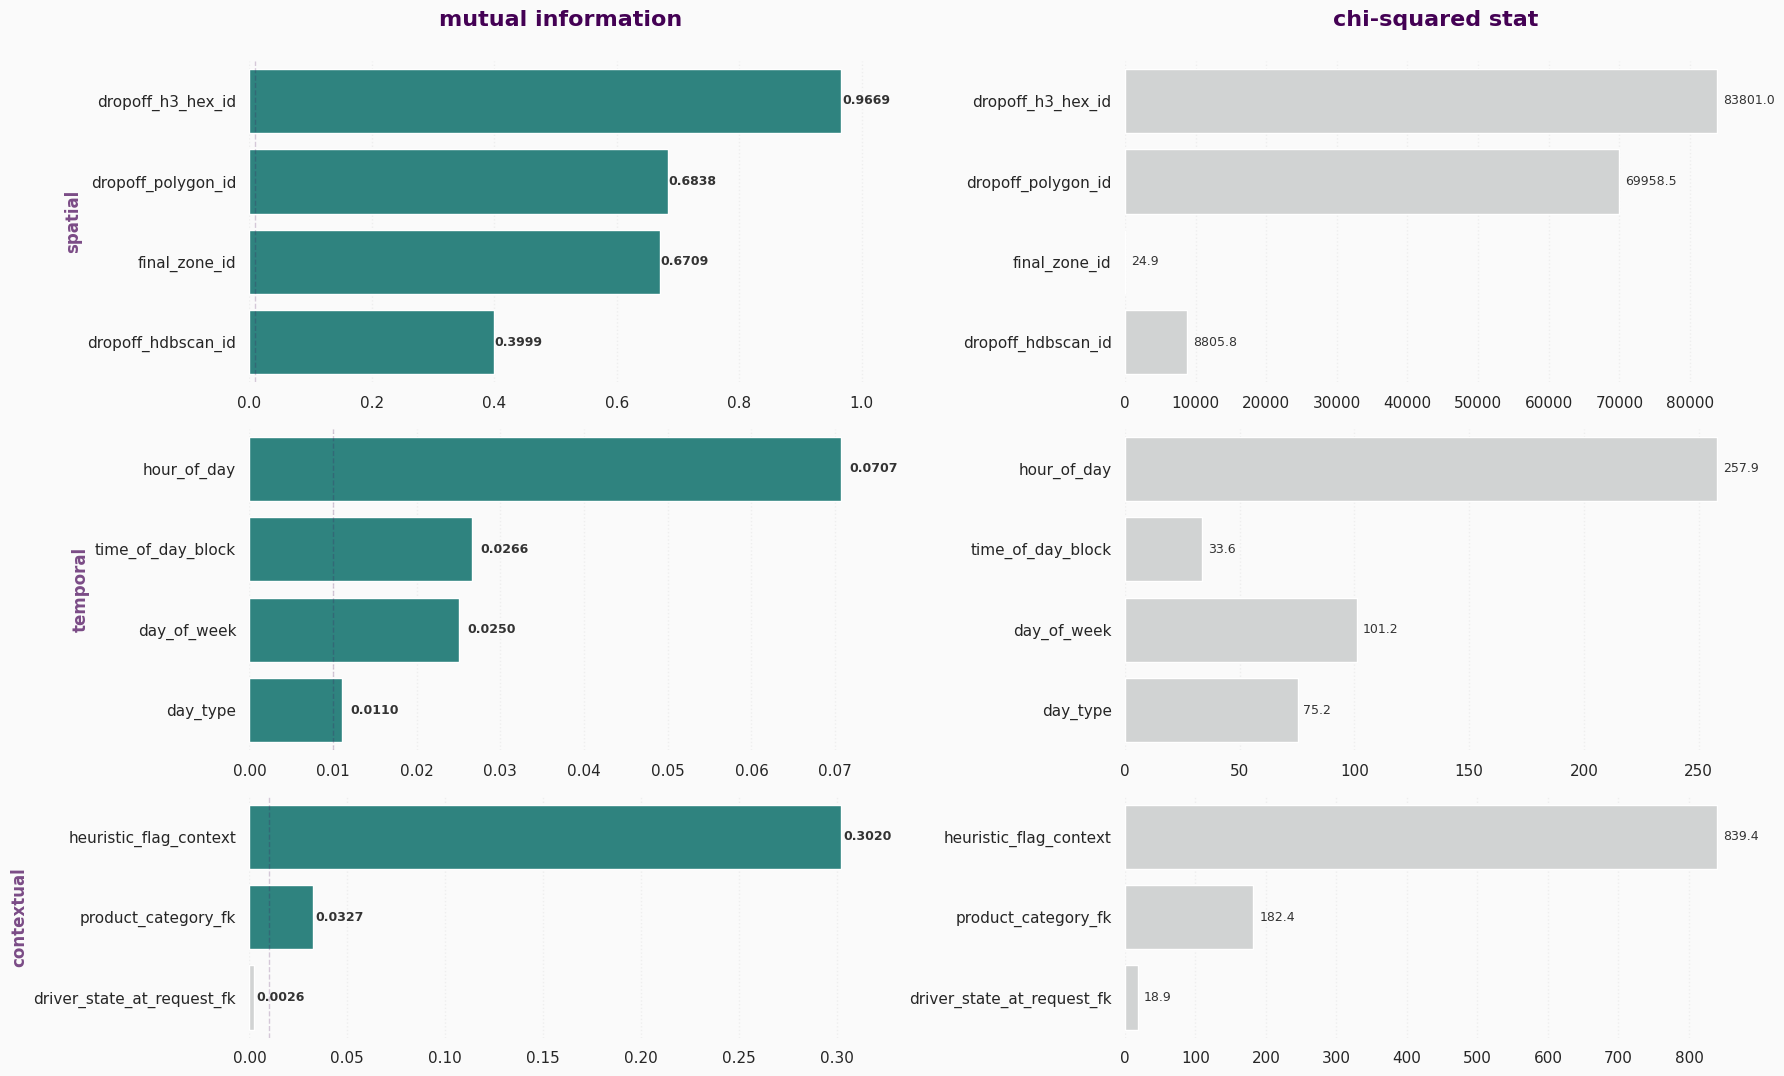
\includegraphics[width=\textwidth]{fig_categorical_audit.png} 
    \caption{Categorical Feature Importance Audit: Mutual Information (Left) and Chi-Squared (Right) scores. The audit exposes the dominance of geospatial topology and the failure of several human-engineered abstractions.}
    \label{fig:categorical_audit}
\end{figure}

The audit identifies \texttt{final\_zone\_id} (MI: 0.671) as the optimal spatial predictor. While high-cardinality grids like H3 with resolution 9 (MI: 0.967) achieve higher raw scores, they risk memorizing the training set. Consolidating 73 polygons into 42 Macro-Zones successfully filtered geometric noise while preserving the variable's predictive power.

The results confirm that raw clock resolution significantly outperforms semantic abstractions. High-resolution features such as \texttt{hour\_of\_day} (MI: 0.071) and \texttt{day\_of\_week} (MI: 0.025) were retained as dominant drivers. Conversely, human-engineered features like \texttt{time\_of\_day\_block} were purged, as their rigid definitions masked critical market variance.

The engineered \texttt{heuristic\_flag\_context} emerged as the primary non-spatial signal (MI: 0.302), validating the "Human-in-the-Loop" extraction phase. In contrast, the Agent's immediate operational state (\textit{Idle vs. On-Trip}) was identified as statistical noise (MI: 0.002) and removed to optimize model focus.

\begin{table}[H]
    \centering
    \small
    \begin{tabularx}{\textwidth}{l l r X}
        \toprule
        \textbf{Domain} & \textbf{Feature} & \textbf{MI Score} & \textbf{Technical Verdict} \\
        \midrule
        \textbf{Spatial} & \texttt{final\_zone\_id} & 0.6709 & \textbf{Keep:} High-resolution zones derived from macro-polygon and cluster coalescence. \\
        \midrule
        \multirow{2}{*}{\textbf{Temporal}} 
        & \texttt{hour\_of\_day} & 0.0707 & \textbf{Keep:} Captures critical high-frequency demand cycles. \\
        & \texttt{day\_of\_week} & 0.0250 & \textbf{Keep:} Preserves unique daily market physics. \\
        \midrule
        \multirow{2}{*}{\textbf{Contextual}} 
        & \texttt{heuristic\_flag\_context} & 0.3020 & \textbf{Keep:} Primary driver; encapsulates strategic intent. \\
        & \texttt{product\_category\_fk} & 0.0327 & \textbf{Keep:} Retained to model service-tier behavioral shifts. \\
        \bottomrule
    \end{tabularx}
    \caption{Final Categorical Feature Set advanced to Supervised Learning ($N \approx 4,760$).}
    \label{tab:cfs_final_set}
\end{table}

\vspace{0.4cm}
\begin{tcolorbox}[
    enhanced, sharp corners, boxrule=0.5pt,
    colframe=gray!50, colback=gray!5,
    left=15pt, right=15pt, top=10pt, bottom=10pt
]
    \sffamily\small
    \textbf{METHODOLOGICAL PIVOT: THE ABLATION STUDY} \\
    \rule{12cm}{0.4pt} \\
    \vspace{0.2cm}
    \rmfamily
    While the initial audit confirmed the high predictive utility of \texttt{heuristic\_flag\_context} (MI: 0.302), a critical review identified this variable as a form of \textbf{Expert Encoding}. Because these manual flags are derived from human backtagging, they constitute an unrealistic "cheat sheet" that would be unavailable in a real-time production environment. 

    \vspace{0.2cm}
    An \textbf{Ablation Study} was executed to remove these manual labels and force the model to rely solely on objective telemetry. The results yielded two project-defining findings:
    \begin{enumerate}[noitemsep, topsep=2pt]
        \item \textbf{Model Robustness:} Predictive performance remained stable, proving that the underlying stateful features (\textit{Silver Palette}) already contained the necessary strategic signal.
        \item \textbf{Explainability Flourish:} Post-ablation \textit{SHAP} analysis revealed a significantly clearer decision DNA. By removing the dominant manual flags, the latent importance of session-progress and accumulated deadhead emerged, providing a more transparent view of the agent's actual behavioral drivers.\footnotemark
    \end{enumerate}
    
    \vspace{0.2cm}
    \textit{Decision: To ensure high-fidelity simulation and production realism, all manual context flags were formally deprecated. The subsequent Algorithmic Tournament was executed exclusively on this purified, autonomous feature space.}
\end{tcolorbox}
\footnotetext{The reader is kindly invited to review the performance \textit{with} heuristic flags in the provided Jupyter Notebooks: \href{https://github.com/your-repo-placeholder}{[GitHub: Project Pienza - Phase 5 Validation]}.}
\vspace{0.4cm}


\subsection{Algorithmic Justification: From First Principles to Ensemble Apex}
To identify the optimal architecture for behavioral cloning, a competitive tournament was executed across five developmental trials. Models were evaluated using the \textbf{F1-Macro} score to ensure predictive balance across the 92\% class imbalance.

A priori selection of high-complexity models was rejected in favor of an iterative tournament designed to establish the statistical performance floor and quantify the non-linear complexity of the Agent’s decision policy. This sequence serves as the formal justification for the eventual deployment of gradient-boosted ensembles.

\begin{itemize}[leftmargin=0.5cm, labelsep=0.3cm]
    \item \textbf{Trial 1: Establishing the Statistical Floor (Naive Bayes).} Gaussian Naïve Bayes was deployed to measure performance under the assumption of feature independence. This trial established the baseline "failure rate" for probabilistic models in a high-imbalance, stateful environment.
    
    \item \textbf{Trial 2: Quantifying the Linear Ceiling (Logistic Regression).} By testing linear decision boundaries across both chronological and stratified splits, the project measured the "Linear Limit" of the dataset. 
    
    \item \textbf{Trial 3: The State-Time Tension (LR Stratified).} This controlled test compared chronological purity against stratified data efficiency. It exposed the "shuffling illusion" common in boutique datasets, where over-optimistic scores can mask a failure to generalize to future market regimes.
    
    \item \textbf{Trial 4: Auditing Non-Linear Logic (Decision Tree).} A single tree was utilized as a "Scout" to audit hard logic splits. This trial provided the empirical proof that raw, uncompressed variables (\textit{LIGA B}) significantly outperformed PCA-abstracted features (\textit{LIGA C}) when navigating non-linear decision rules.
    
    \item \textbf{Trial 5: Architectural Apex (XGBoost).} Armed with the quantified proof of non-linearity and the superiority of raw features, the project deployed a gradient-boosted forest on a consolidated five-week "training gym." This finalized the champion architecture required to capture the nuanced interaction between market physics and agent heuristics.
\end{itemize}

\begin{table}[H]
    \centering
    \scriptsize
    \begin{tabularx}{0.9\textwidth}{l l l c c c}
        \toprule
        \textbf{Trial} & \textbf{Algorithm} & \textbf{Validation Method} & \textbf{LIGA A} & \textbf{LIGA B} & \textbf{LIGA C} \\
        \midrule
        1. Floor & Gaussian NB (Hybrid) & Chronological (Custom) & 0.257 & 0.257 & 0.256 \\
        \addlinespace
        2. Linear & Logistic Regression & Time-Series Split & 0.482 & 0.514 & 0.490 \\
        \addlinespace
        3. Theoretical & Logistic Regression & Stratified K-Fold & 0.687 & 0.716 & 0.691 \\
        \addlinespace
        4. Scout & Decision Tree (d=7) & Time-Series Split & 0.336 & 0.474 & 0.373 \\
        \addlinespace
        \textbf{5. Champion} & \textbf{XGBoost Classifier} & \textbf{Stratified K-Fold} & \textbf{0.760} & \textbf{0.761} & \textit{Retired} \\
        \bottomrule
    \end{tabularx}
    \caption{Performance Ledger: F1-Macro averages across the five developmental trials ($N \approx 4,760$).}
    \label{tab:tournament_ledger}
\end{table}


\subsection{Champion Selection: XGBoost}
\subsection{The ``State vs. Time'' Dilemma}
The ``State vs. Time'' dilemma presented a significant architectural trade-off when modeling on a restricted, short-horizon dataset. Enforcing strict chronological purity---such as sequential walk-forward splits across a mere five-week training window---severely restricts the data volume and the number of learning iterations available to the algorithm. The primary limitation encountered was not an uneven distribution of target classes over time, but rather the data starvation inherent to temporal splits on small datasets, which prevents the model from iteratively refining its logic. 

Fortunately, this structural bottleneck was mitigated by the project's pre-existing feature architecture. Because the Agent's temporal context (e.g., \texttt{hour_of_day}, \texttt{day_of_week}) and behavioral memory (e.g., \texttt{consecutive_rejects}, \texttt{accumulated_deadhead}, \texttt{cumulative_earnings}) had already been explicitly engineered into the feature space, the operative "state" and exact temporal positioning of the agent were intrinsically captured within each independent observation; hence, the algorithm does not require sequential chronological ordering to accurately interpret the context of a decision. Consequently, utilizing Stratified K-Fold cross-validation to shuffle the observations within the training pool does not constitute true data leakage. Instead, it serves as a vital architectural mechanism to maximize data efficiency and iterative learning volume, allowing the model to robustly map the stateful logic before facing an untouched, out-of-time evaluation in Week 6.

\subsection{Model Performance Analysis: The Monolithic Constraint}
The monolithic \texttt{XGBoost} champion was evaluated using purely autonomous features to determine the performance floor of a flat architecture. An audit of the confusion matrix (Figure \ref{fig:ablated_matrix}) identifies a structural failure mode driven by the dataset's class imbalance.

\begin{figure}[H]
    \centering
    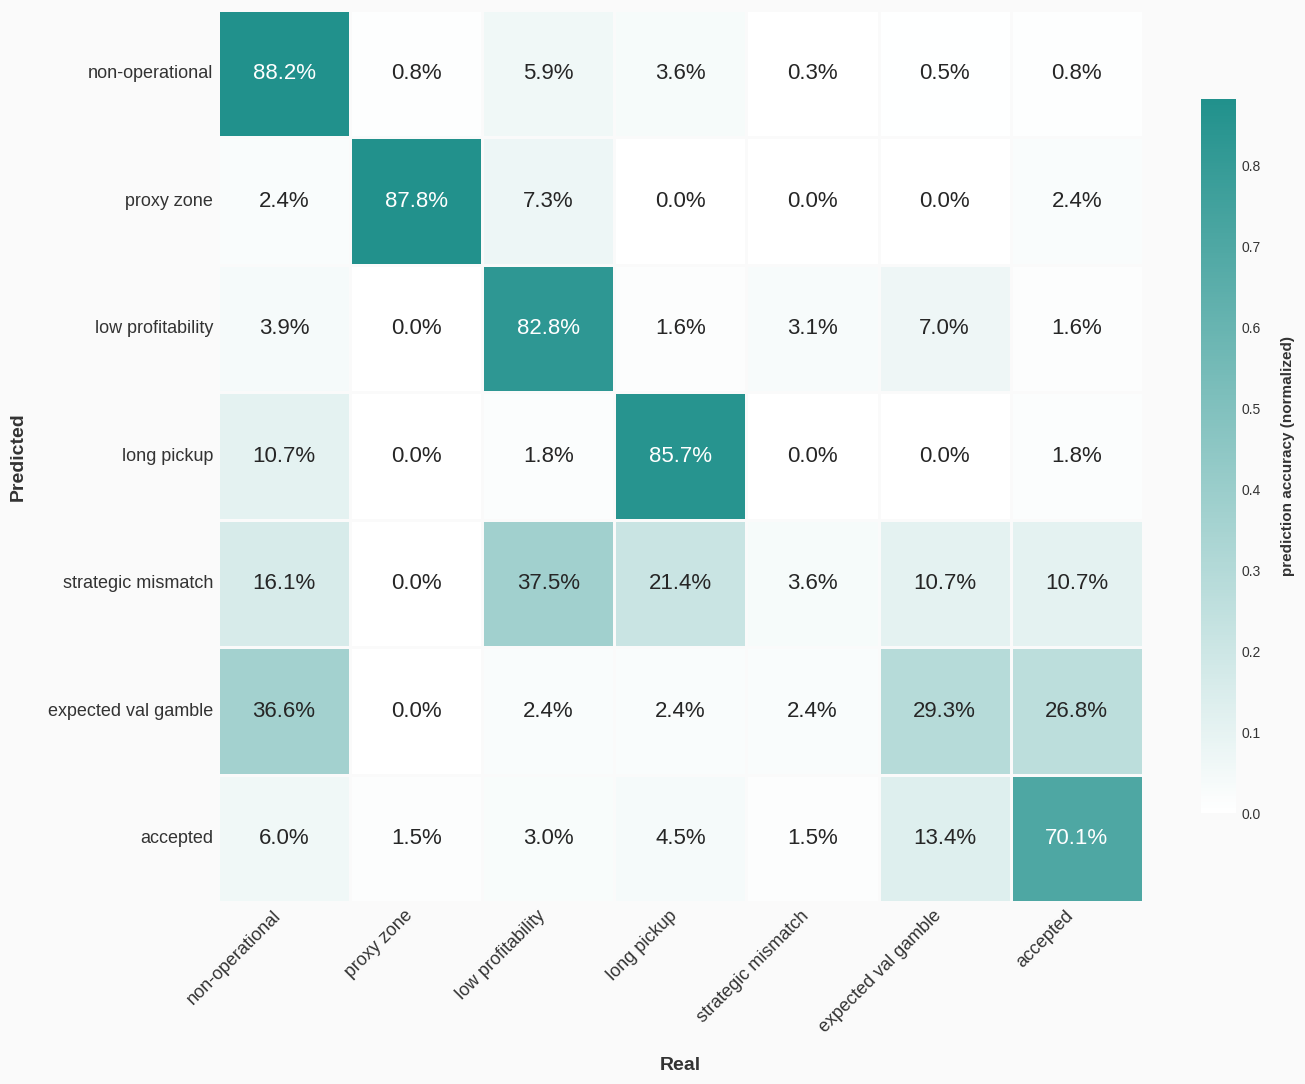
\includegraphics[width=0.85\textwidth]{fig_ablated_matrix.png} 
    \caption{Normalized Confusion Matrix: Monolithic Architecture. While deterministic rejections remain robust, the model fails to differentiate between nuanced strategic classes.}
    \label{fig:ablated_matrix}
\end{figure}

Despite the utilization of balanced class weighting, the monolithic model exhibits a high degree of bias toward the majority classes. Rejections governed by rigid geospatial or economic boundaries—\texttt{non\_operational} and \texttt{low\_profitability}—are predicted with high accuracy ($>82$\%). 

However, these majority classes act as a "gravitational well" for nuanced intent. Strategic rejections (\texttt{strategic\_mismatch} and \texttt{expected\_value\_gamble}) exhibit near-total signal collapse, with 36.6\% of true gambles being incorrectly absorbed by the \texttt{non\_operational} class. This proves that in a flat architecture, deterministic noise cannibalizes the model's ability to learn high-level behavioral patterns.

\subsection{Hierarchical Classification Strategy}
To resolve this, the project pivoted from a monolithic approach to a \textbf{Hierarchical Classification} system. This architecture decomposes the problem into two sequential models:

\begin{enumerate}[noitemsep, topsep=3pt]
    \item \textbf{Layer 1:} The three nuanced classes (\texttt{accepted}, \texttt{strategic\_mismatch}, and \texttt{expected\_value\_gamble}) are collapsed into a single \texttt{THE\_NUANCED\_REST} category, and trained against the majority classes.
    \item \textbf{Layer 2:} A secondary model is trained exclusively on the three nuanced classes so that it can dedicate its full predictive capacity to distinguish between a strategic intent, a gamble, and an acceptance.
\end{enumerate}


\subsection{Layer 1: Isolating Signal from Noise}
To maximize the capture of behavioral intent, the decision threshold for the \texttt{THE\_NUANCED\_REST} class was calibrated at \textbf{0.40}\footnote{To prevent selection bias, Layer 2 performance assessment was executed using 100\% of the manually labeled "nuanced" classes from the holdout set to ensure evaluative isolation.}.  As the confusion matrix (Figure \ref{fig:layer1_matrix}) shows, this optimization achieved a \textbf{70.1\% recall} for the nuanced category, successfully recovering the signal that was previously masked in the flat architecture.

\begin{figure}[H]
    \centering
    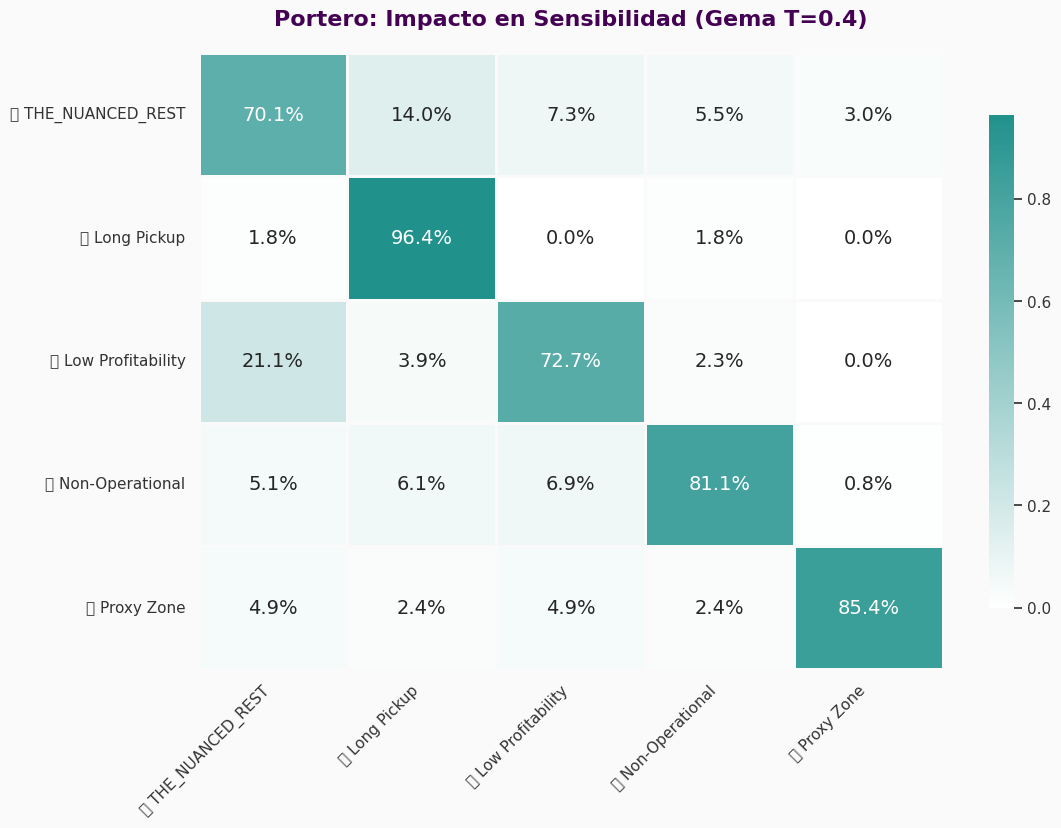
\includegraphics[width=0.85\textwidth]{fig_layer1_matrix_v3.png} 
    \caption{Layer 1 Confusion Matrix ($T=0.40$). The diagonal illustrates the filter's efficiency in isolating noise. Note the 70.1\% successful capture of the nuanced signal.}
    \label{fig:layer1_matrix}
\end{figure}

With a \textbf{Macro F1-score of 0.76}, the classification report (Table \ref{tab:layer1_report}) confirms the successful removal of low-level noise, specifically identifying \texttt{non\_operational} events with 96\% precision while maintaining a \textbf{0.81 Macro Recall}. 

\begin{table}[H]
    \centering
    \small
    \begin{tabular}{l c c c r}
        \toprule
        \textbf{Class Label} & \textbf{Precision} & \textbf{Recall} & \textbf{F1-Score} & \textbf{Support} \\
        \midrule
        \texttt{THE\_NUANCED\_REST} & 0.70 & 0.70 & 0.70 & 164 \\ \addlinespace[2pt]
        \texttt{long\_pickup}        & 0.50 & 0.96 & 0.66 & 56  \\ \addlinespace[2pt]
        \texttt{low\_profitability}  & 0.69 & 0.73 & 0.71 & 128 \\ \addlinespace[2pt]
        \texttt{non\_operational}     & 0.96 & 0.81 & 0.88 & 391 \\ \addlinespace[2pt]
        \texttt{dropoff\_proxy}      & 0.81 & 0.85 & 0.83 & 41  \\ \addlinespace[4pt]
        \midrule
        \textbf{Macro Average}       & \textbf{0.73} & \textbf{0.81} & \textbf{0.76} & \textbf{780} \\
        \bottomrule
    \end{tabular}
    \caption{Layer 1 Classification Report: Triage aggregates for noise filtration.}
    \label{tab:layer1_report}
\end{table}

\subsubsection{Discriminatory Power: ROC and Precision-Recall Analysis}

While ROC-AUC measures discriminatory capacity in balanced datasets, the significant class imbalance in this project necessitates the implementation of Precision-Recall (PR) analysis. Unlike the ROC framework, PR-AUC ignores easily predicted True Negatives, focusing strictly on the model's accuracy in capturing rare positive signals. Analysis of the \texttt{THE_NUANCED_REST} class (Figure \ref{fig:layer1_curves}) yields an \textbf{AUC of 0.87} and an \textbf{Average Precision of 0.76}. Overall, a \textbf{Macro AP of 0.7969}, shows a robust stability for the nuanced signal; these results ensure that inputs to the subsequent layer are statistically prioritized.


\begin{figure}[H]
    \centering
    \begin{subfigure}[b]{0.49\textwidth}
        \centering
        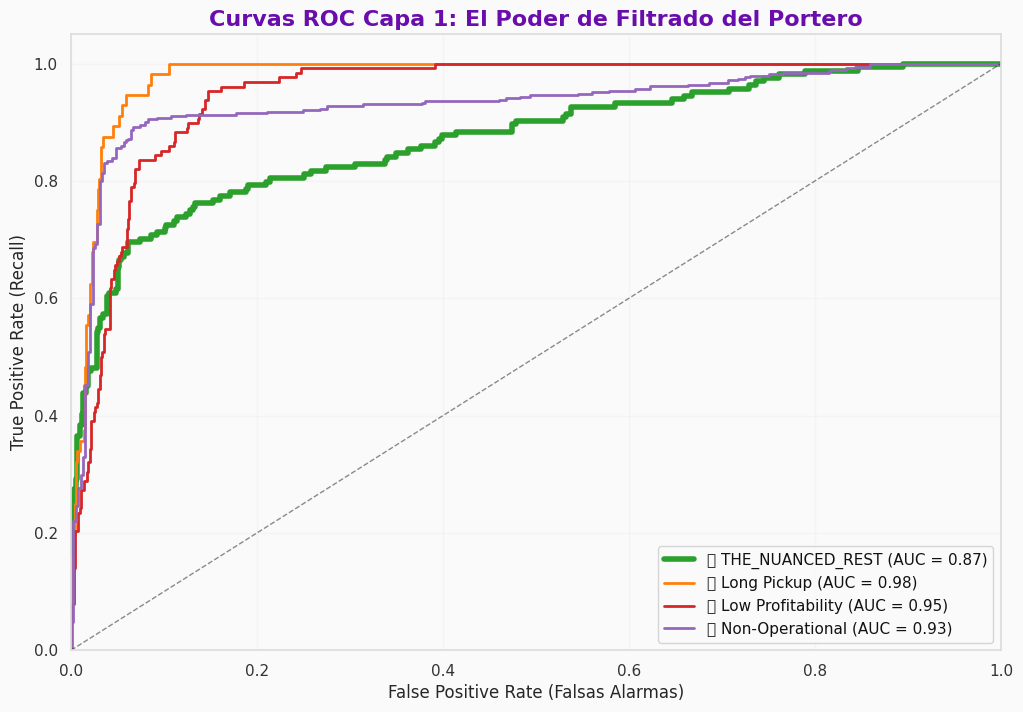
\includegraphics[width=\textwidth]{fig_layer1_roc.png} 
        \caption{ROC Curves: Filtering Power}
        \label{fig:layer1_roc}
    \end{subfigure}
    \hfill
    \begin{subfigure}[b]{0.49\textwidth}
        \centering
        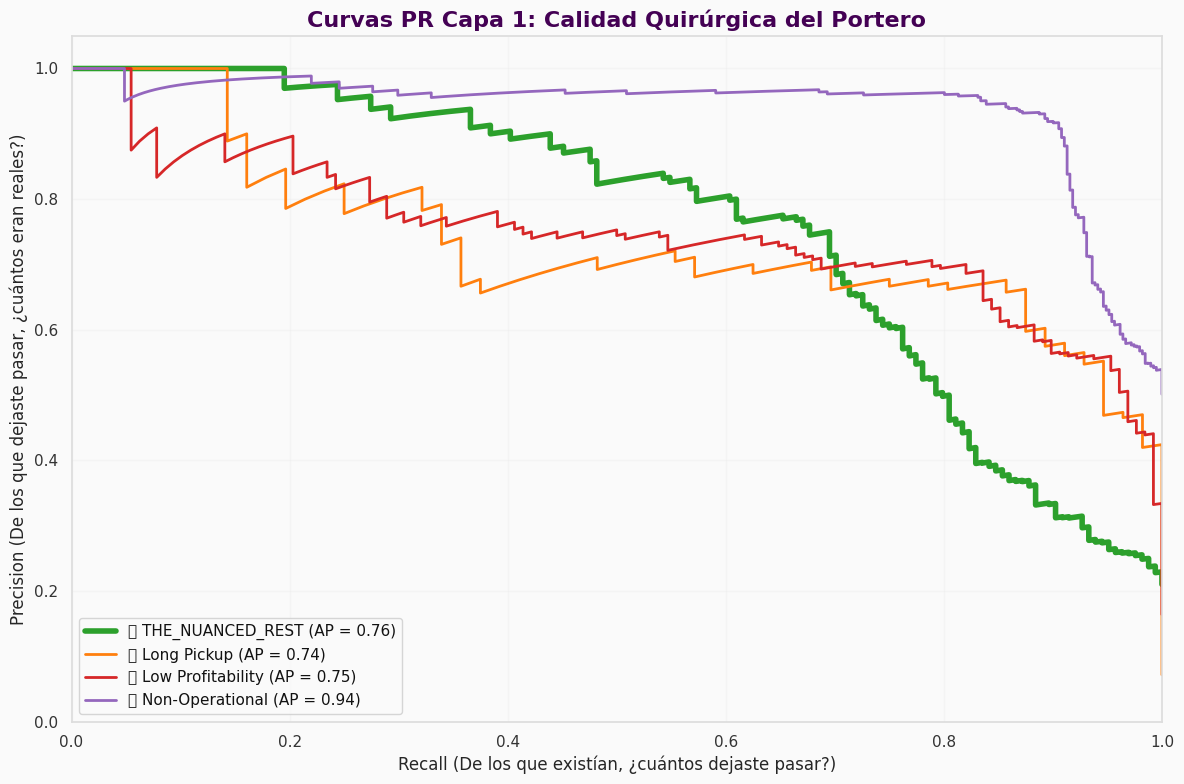
\includegraphics[width=\textwidth]{fig_layer1_pr.png} 
        \caption{PR Curves: Precision Stability}
        \label{fig:layer1_pr}
    \end{subfigure}
    \caption{Layer 1 Performance Curves. The high AUC for deterministic rejections confirms the model's efficiency in protecting the subsequent layer from data contamination.}
    \label{fig:layer1_curves}
\end{figure}

\begin{table}[H]
    \centering
    \small
    \begin{tabular}{l c l}
        \toprule
        \textbf{Aggregate Metric} & \textbf{Value} & \textbf{Technical Verdict} \\
        \midrule
        Macro AUC-ROC & \textbf{0.9415} & \textbf{EXCELLENT:} Near-total separation of deterministic noise. \\ \addlinespace[2pt]
        Macro Average Precision (AP) & \textbf{0.7969} & \textbf{ROBUST:} High precision stability for the nuanced signal. \\
        \bottomrule
    \end{tabular}
    \caption{Layer 1 Macro Performance Summary.}
    \label{tab:layer1_macro_summary}
\end{table}





\subsubsection{Generalization Audit: Learning Curve Analysis}
To ensure model stability and identify data constraints, a Learning Curve audit was executed (Figure \ref{fig:layer1_learning}). This analysis monitors the performance delta between training and validation scores as the training sample size ($N$) increases, identifying the transition from high-variance noise to stable logic.

\begin{figure}[H]
    \centering
    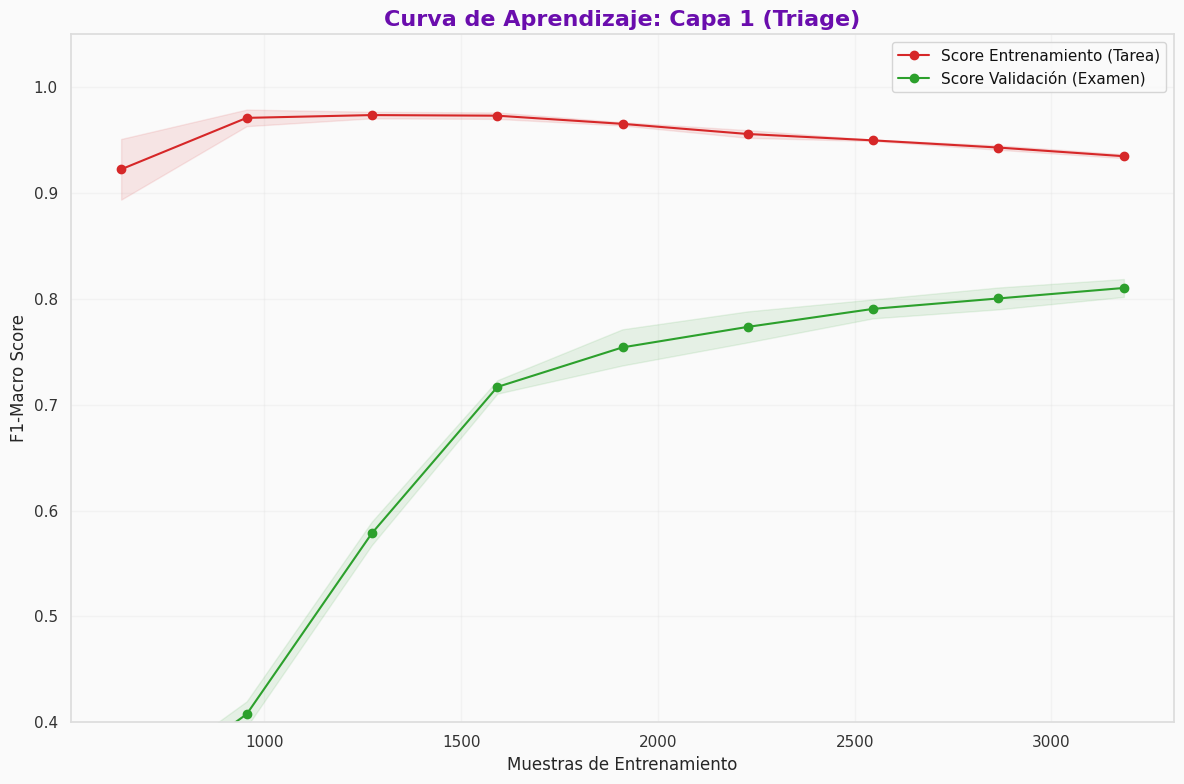
\includegraphics[width=0.85\textwidth]{fig_layer1_learning.png} 
    \caption{Layer 1 Learning Curve. The narrowing delta between the training and validation scores indicates successful logic convergence, while the upward trajectory of the validation curve suggests a data-starved state.}
    \label{fig:layer1_learning}
\end{figure}

\begin{table}[H]
    \centering
    \small
    \begin{tabularx}{0.85\textwidth}{l c X}
        \toprule
        \textbf{Diagnostic Metric} & \textbf{Value} & \textbf{Technical Verdict} \\
        \midrule
        Final Validation Score & \textbf{0.8103} & \textbf{STABLE:} Model generalizes effectively to unseen data. \\ \addlinespace[2pt]
        Generalization Gap & 0.1245 & \textbf{MODERATE:} Variance is narrowing as training volume increases. \\
        \bottomrule
    \end{tabularx}
    \caption{Learning Curve Diagnostic Summary.}
    \label{tab:layer1_learning_summary}
\end{table}

The persistent upward slope of the validation curve identifies a \textbf{data-starved state}; while the current model is operationally valid, the performance ceiling remains active, indicating that accuracy would likely scale linearly with additional ground-truth samples.




\subsubsection{SHAP DNA}
To interpret the internal logic of the first-tier filter, a SHAP (Shapley Additive exPlanations) audit was performed on the \texttt{THE\_NUANCED\_REST} class (Figure \ref{fig:layer1_shap}). This analysis identifies the features that qualify an offer for Layer 2 evaluation versus those that drive a deterministic rejection.

\begin{figure}[H]
    \centering
    
\includegraphics[width=0.85\textwidth]{fig_layer1_shapv2.png} 
    \caption{Layer 1 Signal Drivers. Teal bars indicate features that push an offer into the ``Nuanced'' category for evaluation; gray bars indicate features that drive a deterministic rejection.}
    \label{fig:layer1_shap}
\end{figure}

The SHAP audit reveals the structural separation between deterministic rejections and the nuanced selection signal. The triage logic is governed by three primary mechanics:

\begin{itemize}[noitemsep, topsep=3pt]
    \item \textbf{The Topographic Filter (Exclusion):} The primary drivers for rejection are geospatial. Destinations in the \texttt{Unassigned Area} ($-0.332$) and proxy zones like \texttt{Roma/Condesa} ($-0.196$) trigger immediate exclusion. This confirms that at the first tier, the Agent prioritizes "Where" over "How much".
    
    \item \textbf{The Traffic Chaser Heuristic (Inclusion):} Contrary to standard assumptions, high congestion serves as a positive inclusion signal. The \texttt{historical\_rolling\_avg\_traffic\_index} ($+0.144$) and \texttt{traffic\_index} ($+0.106$) push offers into the Nuanced category. This validates the strategy of targeting high-friction market states to secure EPH premiums that are often absent in fluid, low-demand regimes.
    
    \item \textbf{Volatility vs. Friction:} While known traffic is desirable, unpredicted risk is not. The \texttt{traffic\_volatility\_index\_ml} ($-0.068$) acts as a negative driver. Rejection is triggered not by friction itself, but by the \textbf{uncertainty} of the algorithm's prediction. High volatility signals the risk of operational margin erosion. This justifies the late-stage engineering of the volatility suite following the causal inference audit.
\end{itemize}




\subsection{Layer 2: Nuance Engine}
The second stage of the hierarchy resolves the distinctions between strategic rejections and final acceptance. By operating exclusively on the high-signal sub-universe, the engine achieves separation between complex decision states (Figure \ref{fig:layer2_matrix}).

\begin{figure}[H]
    \centering
    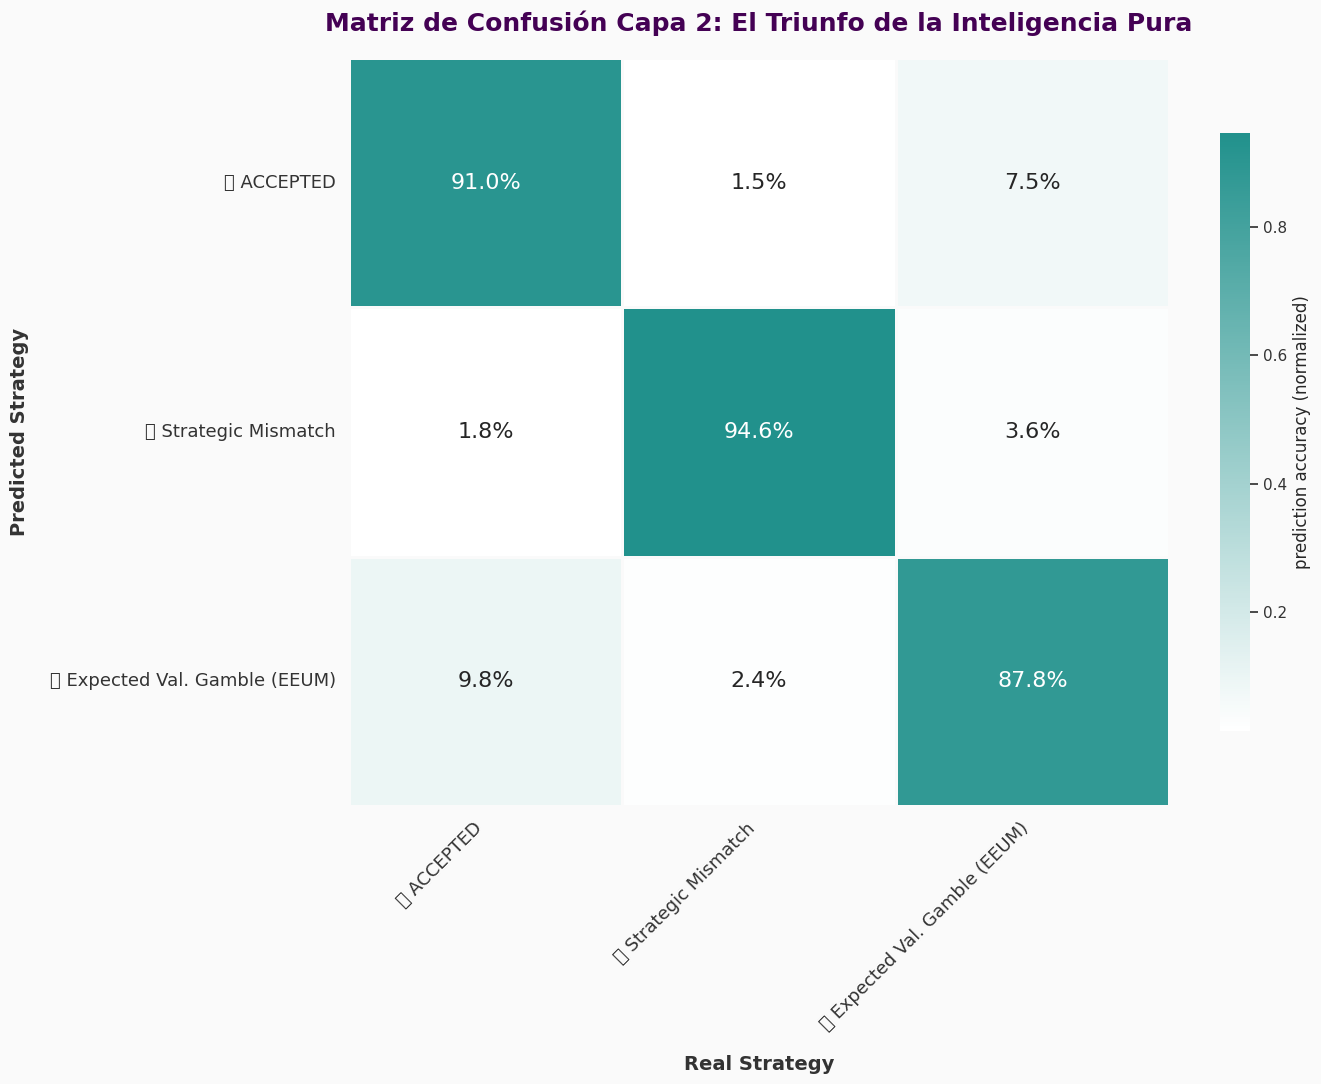
\includegraphics[width=0.85\textwidth]{fig_layer2_matrixv2.png} 
    \caption{Layer 2 Confusion Matrix. The model separates nuanced classes with high precision after the removal of deterministic noise.}
    \label{fig:layer2_matrix}
\end{figure}

The model achieved a \textbf{Macro F1-score of 0.91} on the holdout set ($N=164$). The result, detailed in Table \ref{tab:layer2_report}, represents a lift over the monolithic baseline and confirms that isolating intent from deterministic noise enables the engine to replicate expert policy. 

\begin{table}[H]
    \centering
    \small
    \begin{tabular}{l c c c r}
        \toprule
        \textbf{Class Label} & \textbf{Precision} & \textbf{Recall} & \textbf{F1-Score} & \textbf{Support} \\
        \midrule
        \texttt{ACCEPTED}               & 0.92 & 0.91 & 0.92 & 67 \\ \addlinespace[2pt]
        \texttt{strategic\_mismatch}    & 0.96 & 0.95 & 0.95 & 56 \\ \addlinespace[2pt]
        \texttt{expected\_value\_gamble}& 0.84 & 0.88 & 0.86 & 41 \\ \addlinespace[4pt]
        \midrule
        \textbf{Macro Average}          & \textbf{0.91} & \textbf{0.91} & \textbf{0.91} & \textbf{164} \\
        \bottomrule
    \end{tabular}
    \caption{Layer 2 Classification Report: Strategic decision cloning performance.}
    \label{tab:layer2_report}
\end{table}


\subsubsection{Discriminatory Power: ROC and Precision-Recall Analysis}
The ROC-AUC and PR-AUC analyses (Figure \ref{fig:layer2_curves}) identify the successful neutralization of the signal-masking effect. All decision classes---including the \texttt{expected\_value\_gamble} (AUC: 0.97)---reach performance levels near the theoretical maximum. 

\begin{figure}[H]
    \centering
    \begin{subfigure}[b]{0.49\textwidth}
        \centering
        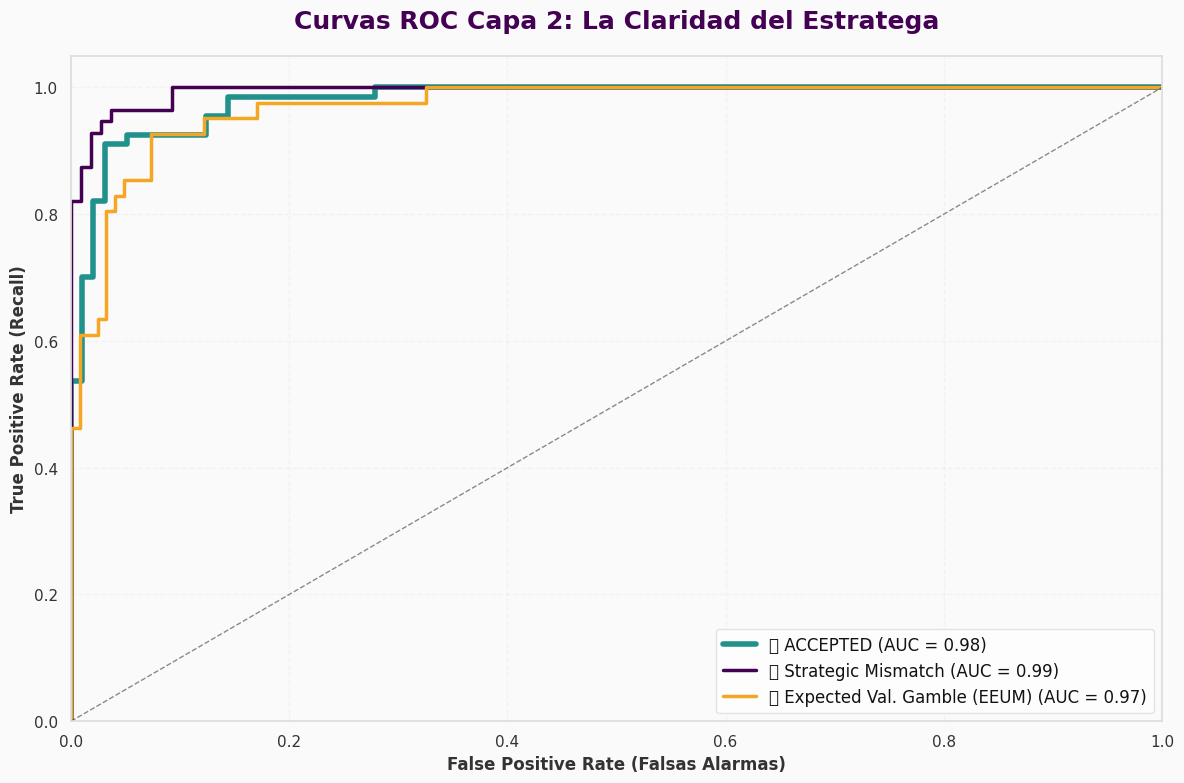
\includegraphics[width=\textwidth]{fig_layer2_roc.png} 
        \caption{ROC Curves: Separation Capacity}
        \label{fig:layer2_roc}
    \end{subfigure}
    \hfill
    \begin{subfigure}[b]{0.49\textwidth}
        \centering
        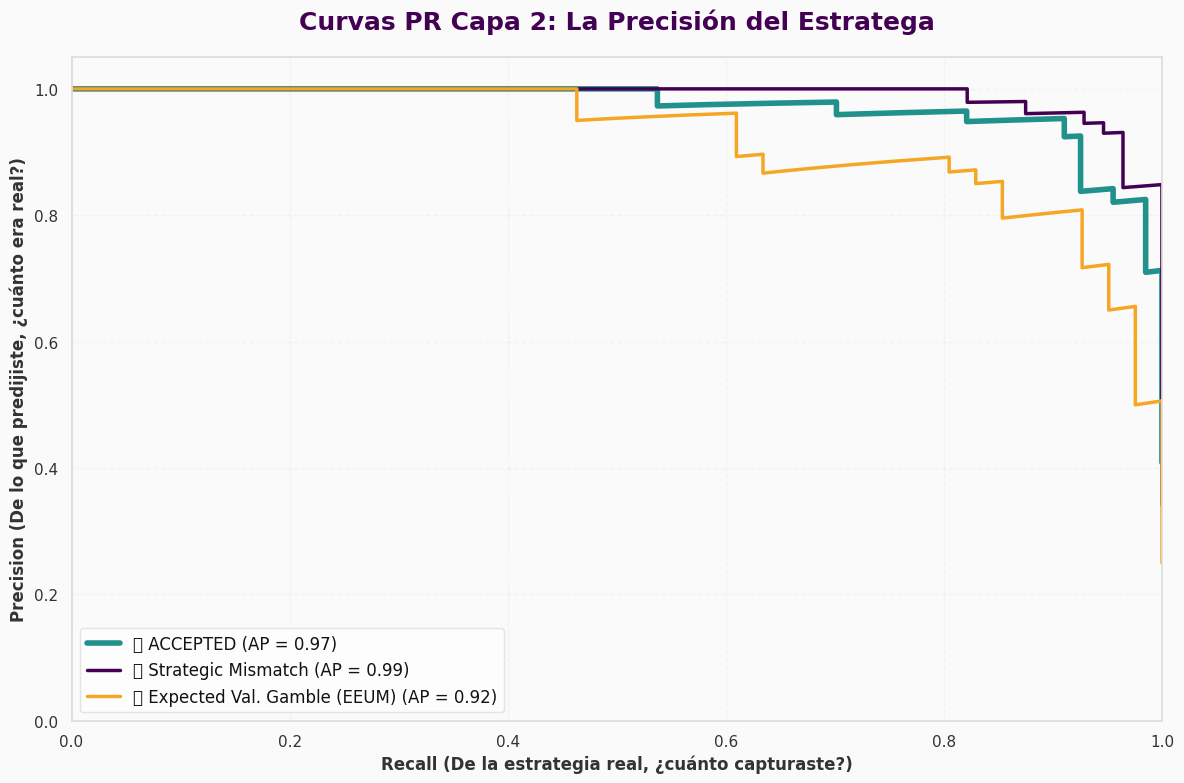
\includegraphics[width=\textwidth]{fig_layer2_pr.png} 
        \caption{PR Curves: Decision Stability}
        \label{fig:layer2_pr}
    \end{subfigure}
    \caption{Layer 2 Performance Curves. The proximity of the functions to the upper-right coordinate confirms high fidelity in replicating expert intent.}
    \label{fig:layer2_curves}
\end{figure}

\begin{table}[H]
    \centering
    \small
    \begin{tabular}{l c l}
        \toprule
        \textbf{Aggregate Metric} & \textbf{Value} & \textbf{Technical Verdict} \\
        \midrule
        Macro AUC-ROC & \textbf{0.9814} & \textbf{ELITE:} Near-total separation of nuanced intent. \\ \addlinespace[2pt]
        Macro Average Precision (AP) & \textbf{0.9613} & \textbf{ELITE:} Exceptional precision stability. \\ \addlinespace[2pt]
        \texttt{ACCEPTED} Class Uplift & \textbf{+56.3 pts} & \textbf{SIGNIFICANT:} Model AP (97.2\%) vs. Random Baseline (40.9\%). \\
        \bottomrule
    \end{tabular}
    \caption{Layer 2 Macro Performance and Class-Specific Uplift Summary.}
    \label{tab:layer2_macro_summary}
\end{table}

The most significant result is the PR stability of the \texttt{ACCEPTED} class. As shown in (Table \ref{tab:layer2_macro_summary}), achieving an Average Precision of \textbf{97.2\%} represents a 56.3-point lift over the random baseline. 

\subsubsection{Generalization Audit: The Variance-Bias Constraint}
Although initial results appeared promising, holdout testing revealed that the Layer 2 model had overfitted rather than generalized to unseen data. Due to the limited sample size ($N=787$), the model suffered from curse of dimensionality. As shown in the learning curves (Figure \ref{fig:layer2_learning}), the high feature count relative to the small subset size compromised stability. To resolve this, a refined ``lightweight'' configuration utilizing only six core features was engineered (Table \ref{tab:l2_light_features}).

\begin{table}[H]
    \centering
    \small
    \begin{tabular}{l}
        \toprule
        \textbf{Feature Name} \\
        \midrule
        \texttt{session\_progress\_ratio} \\ \addlinespace[2pt]
        \texttt{total\_acc\_deadhead\_sec} \\ \addlinespace[2pt]
        \texttt{cycle\_rolling\_avg\_spread} \\ \addlinespace[2pt]
        \texttt{eph\_operational\_index} \\ \addlinespace[2pt]
        \texttt{cycle\_cum\_net\_earnings} \\ \addlinespace[2pt]
        \texttt{home\_vector\_alignment\_score} \\
        \bottomrule
    \end{tabular}
    \caption{The distilled feature set for the lightweight model.}
    \label{tab:l2_light_features}
\end{table}

\begin{figure}[H]
    \centering
    \begin{subfigure}[b]{0.49\textwidth}
        \centering
        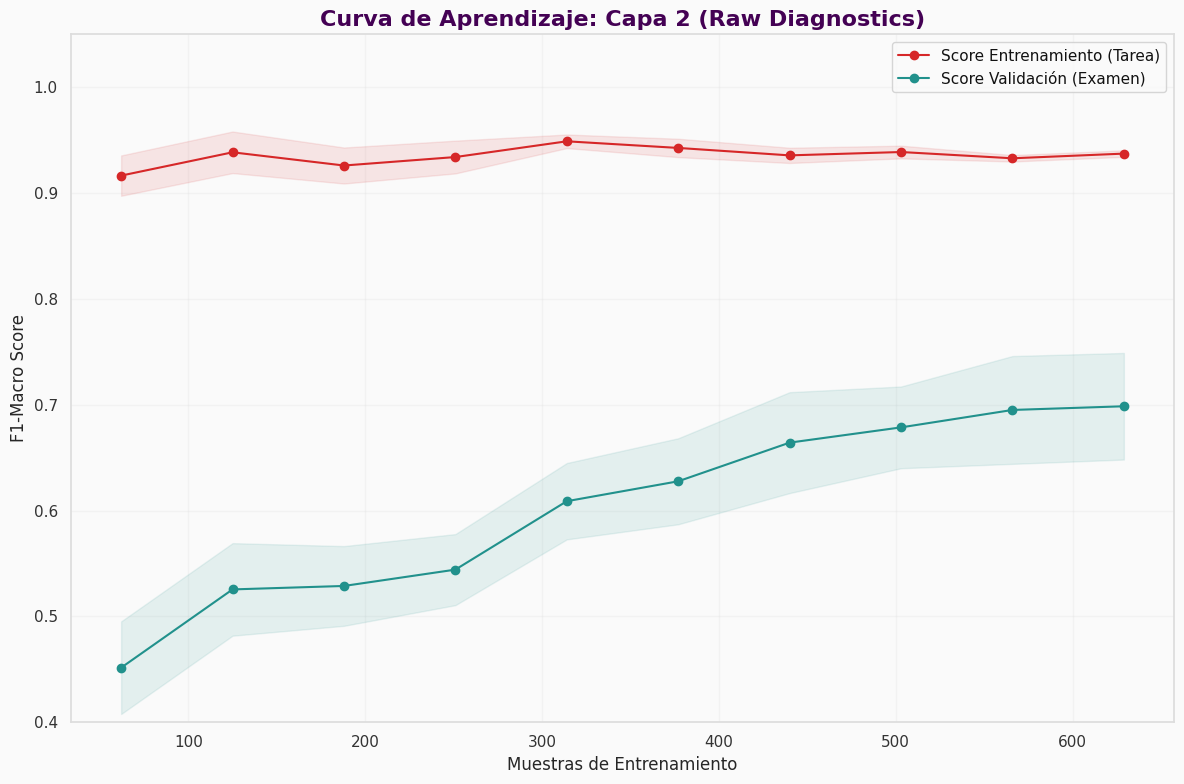
\includegraphics[width=\textwidth]{fig_layer2_learning_raw.png} 
        \caption{Full Feature Set (Raw)}
        \label{fig:l2_learn_raw}
    \end{subfigure}
    \hfill
    \begin{subfigure}[b]{0.49\textwidth}
        \centering
        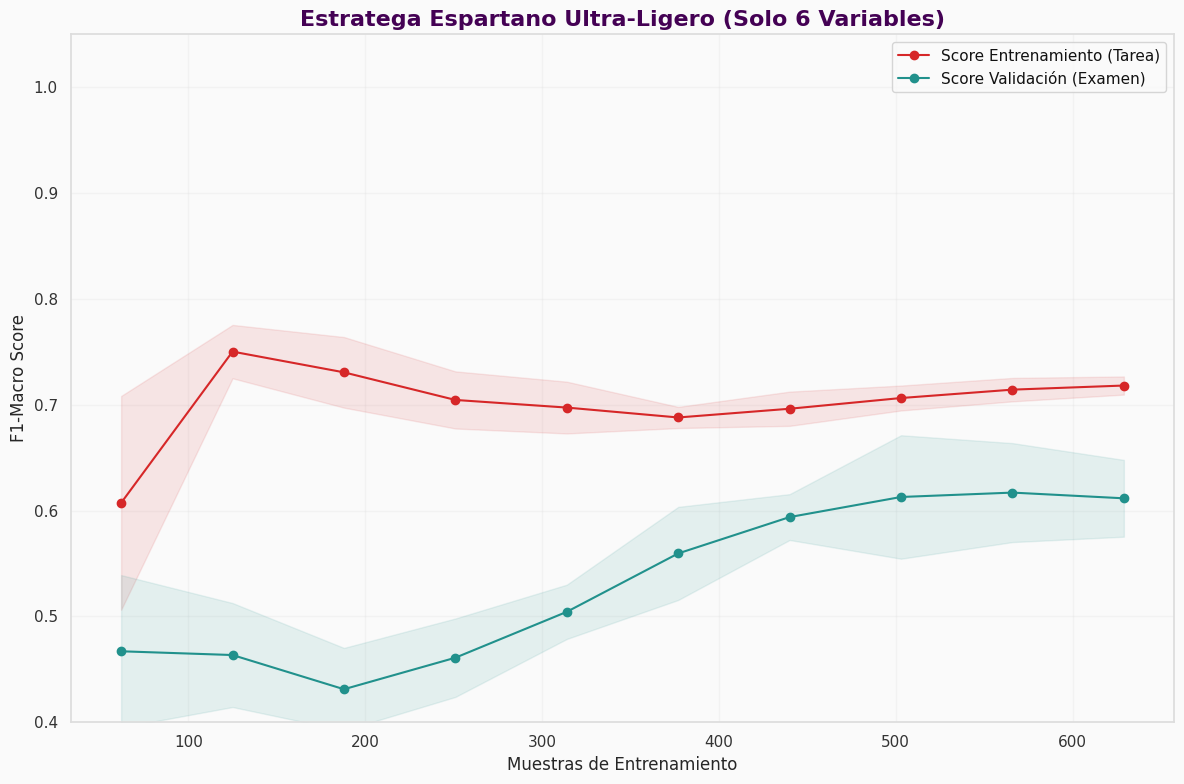
\includegraphics[width=\textwidth]{fig_layer2_learning_light.png} 
        \caption{Lightweight Matrix (6 Features)}
        \label{fig:l2_learn_light}
    \end{subfigure}
    \caption{Layer 2 Generalization Audit. The comparison illustrates the tension between capturing intent (high variance) and achieving stable generalization (high bias).}
    \label{fig:layer2_learning}
\end{figure}



\begin{table}[H]
    \centering
    \small
    \begin{tabularx}{\textwidth}{l c c c X}
        \toprule
        \textbf{Configuration} & \textbf{Train F1} & \textbf{Val F1} & \textbf{Gap ($\Delta$)} & \textbf{Diagnostic Verdict} \\
        \midrule
        Full Feature Set & 0.9373 & \textbf{0.6986} & 0.2387 & \textbf{HIGH VARIANCE:} The model overfitted to the training set. \\ \addlinespace[4pt]
        Lightweight Matrix & 0.7182 & \textbf{0.6116} & \textbf{0.1066} & \textbf{HIGH BIAS:} A 10\% gap means the model generalized better, with the tradeoff of losing predictive capacity. \\
        \bottomrule
    \end{tabularx}
    \caption{Layer 2 Robustness Audit: Comparative performance and generalization gap.}
    \label{tab:layer2_learning_summary}
\end{table}





FALTA (Sigue): SHAP y coliseo





\subsection{Layer 2: The Strategist (Nuance Modeling)}
% ... (Mantener texto introductorio) ...

\begin{figure}[H]
    \centering
    \textcolor{red}{\textbf{[PLACEHOLDER: ACTUALIZAR MATRIZ CAPA 2]}} \\
    \textit{Current state: fig\_layer2\_matrix.png}
\end{figure}

\begin{figure}[H]
    \centering
    \begin{subfigure}[b]{0.45\textwidth}
        \centering
        \textcolor{red}{\fbox{Classification Report}}
        \caption{Precision-Recall Per Class}
    \end{subfigure}
    \hfill
    \begin{subfigure}[b]{0.45\textwidth}
        \centering
        \textcolor{red}{\fbox{ROC-AUC Curve}}
        \caption{Discriminatory Power}
    \end{subfigure}
    \vspace{0.5cm}
    \begin{subfigure}[b]{0.45\textwidth}
        \centering
        \textcolor{red}{\fbox{Precision-Recall Curve}}
        \caption{Threshold Stability}
    \end{subfigure}
    \hfill
    \begin{subfigure}[b]{0.45\textwidth}
        \centering
        \textcolor{red}{\fbox{Learning Curve}}
        \caption{Generalization Audit}
    \end{subfigure}
    \caption{Layer 2 Diagnostic Suite: Performance metrics for behavioral policy cloning.}
\end{figure}























\subsubsection{Strategic DNA: Feature Drivers for Layer 2}
To interpret the internal logic of the Strategist model, a SHAP contribution analysis was performed across the three nuanced strategic classes (Figure \ref{fig:layer2_shap_dna}). This assessment quantifies the directional impact of features on the final classification.

\begin{figure}[H]
    \centering
    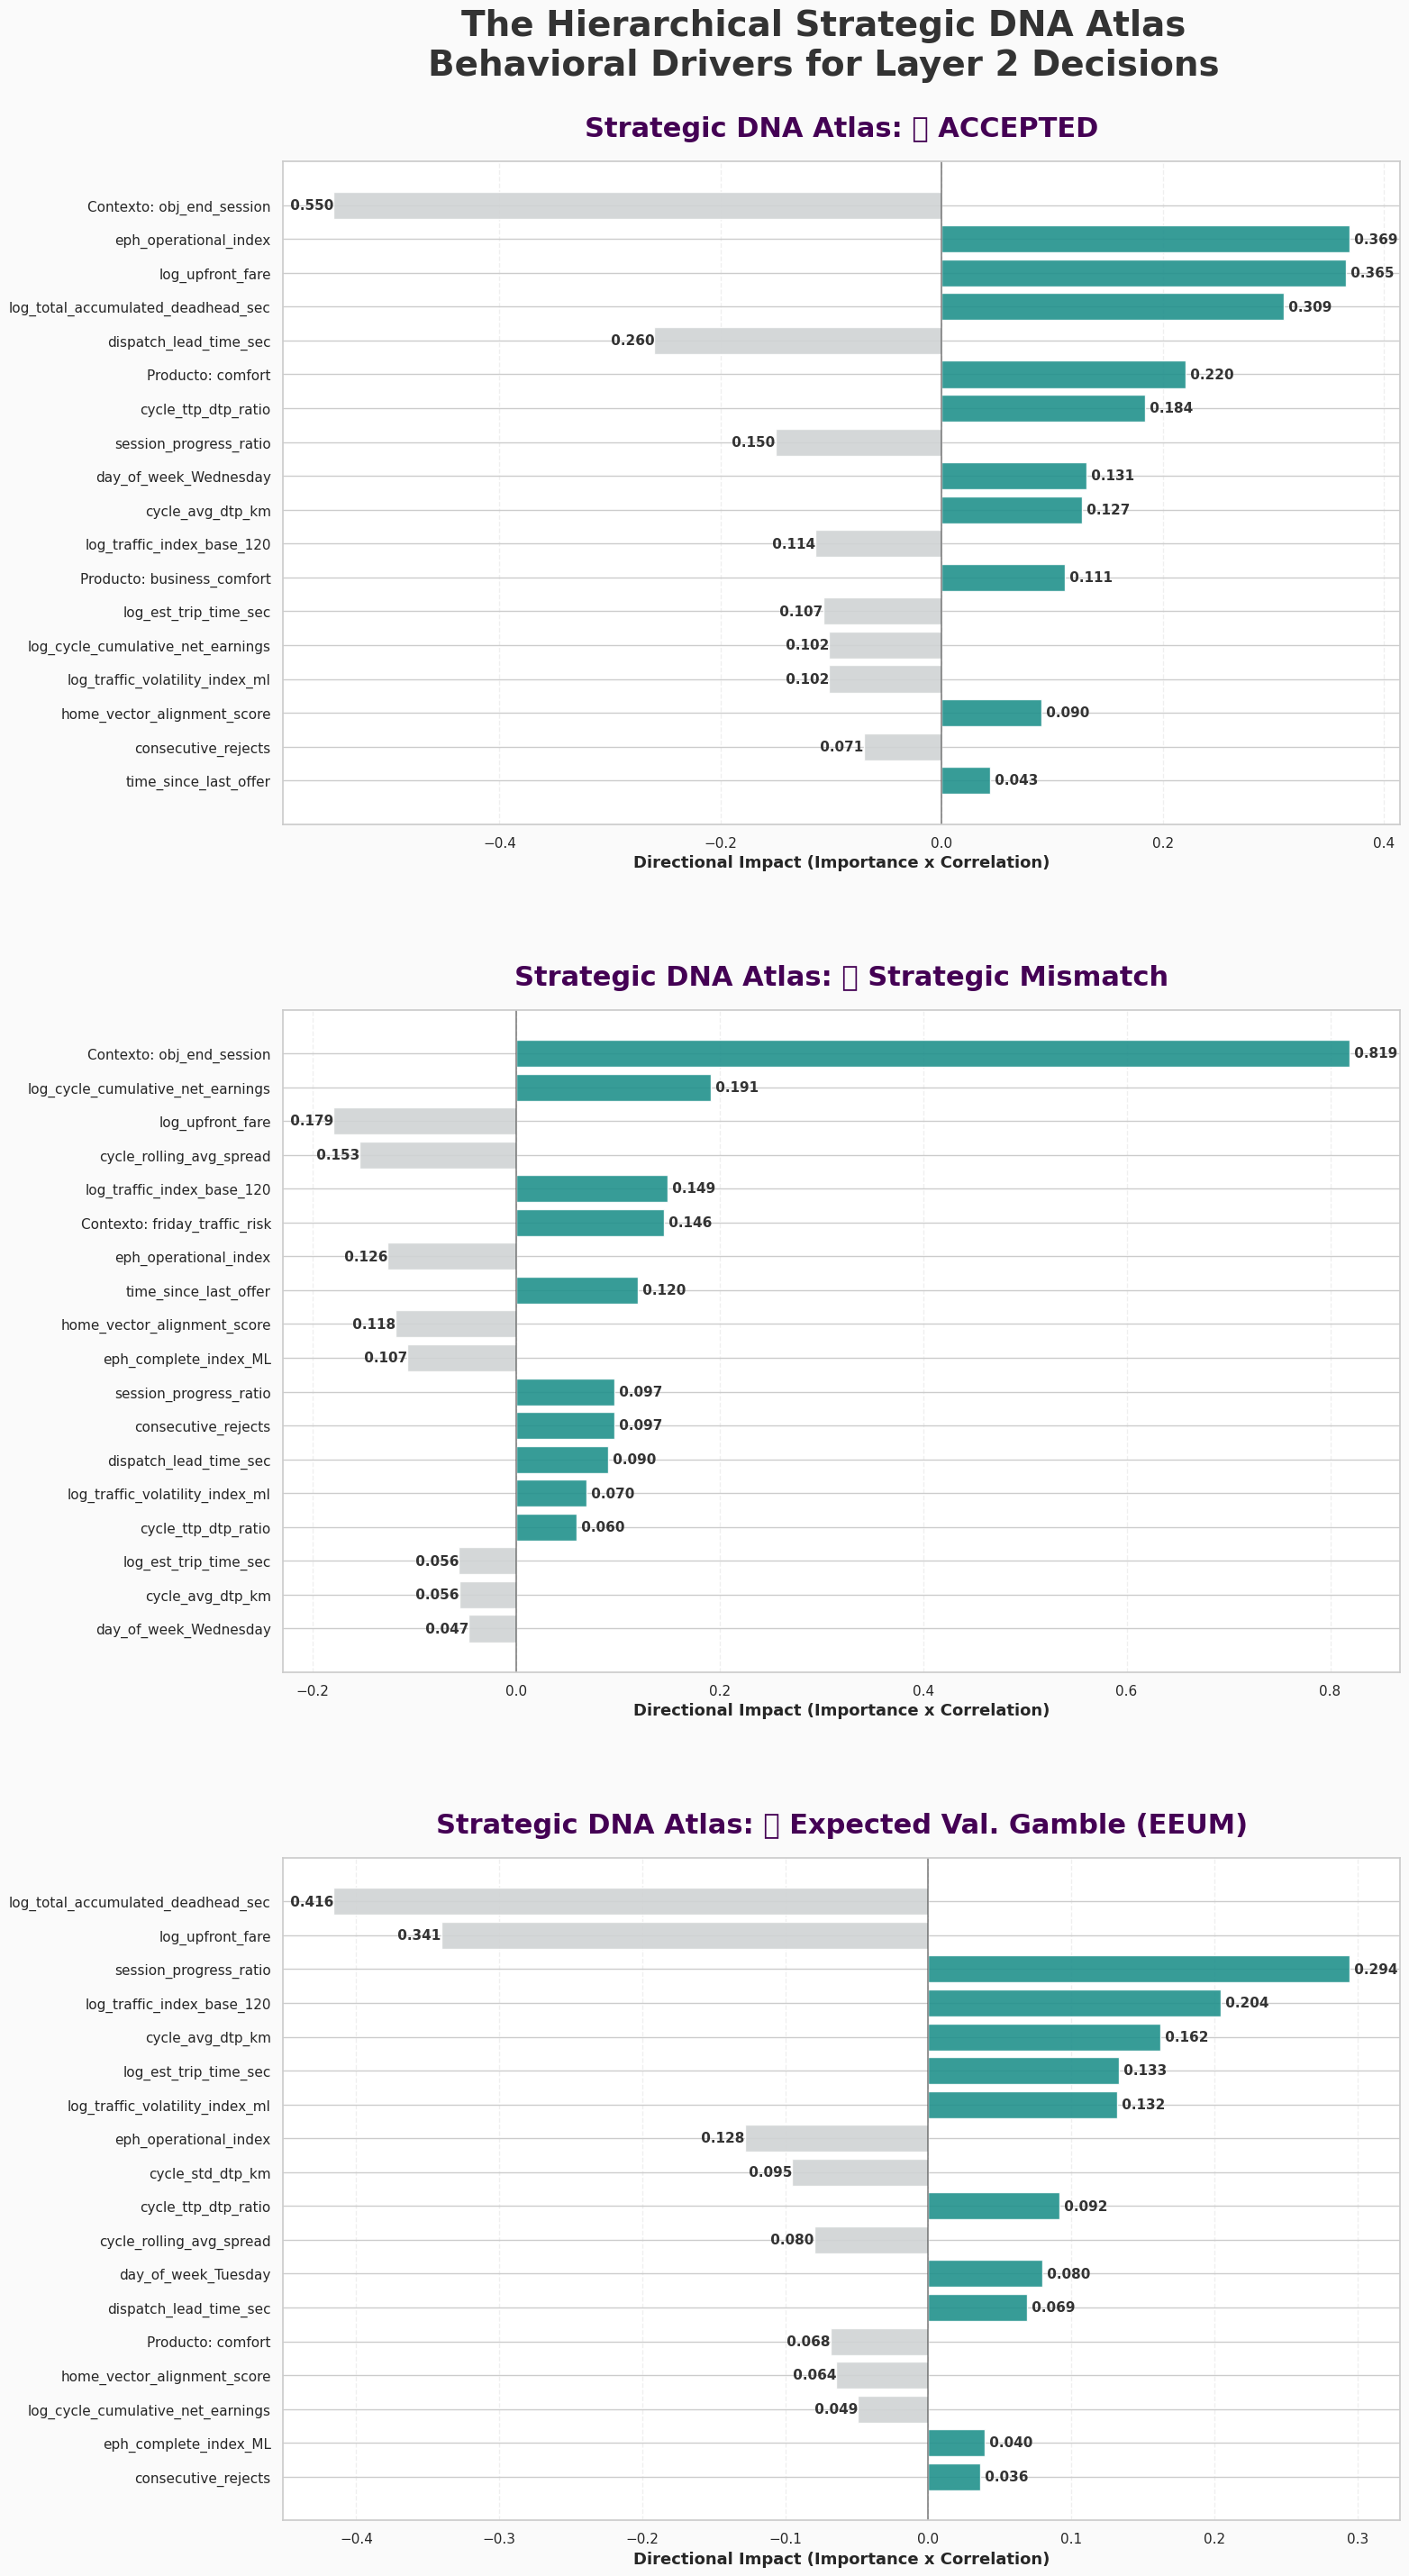
\includegraphics[width=0.6\textwidth]{fig_layer2_shap_dna.png} 
    \caption{Hierarchical Strategic DNA Atlas: Feature contributions for Layer 2 decision classes. Teal bars indicate a positive contribution to class probability; Gray bars indicate a negative contribution.}
    \label{fig:layer2_shap_dna}
\end{figure}

The analysis reveals three primary behavioral mechanics that govern the expert agent's high-level strategy:

\begin{itemize}[noitemsep, topsep=3pt]
    \item \textbf{The Sunk Cost Mechanic (Accepted):} While \texttt{upfront\_fare} and \texttt{eph\_operational\_index} are the expected financial drivers, \texttt{log\_total\_accumulated\_deadhead\_sec} serves as a powerful positive predictor ($+0.309$). This provides empirical proof of a ``Sunk Cost'' effect: as uncompensated search time increases, the Agent's selectivity threshold decays, leading to a higher probability of acceptance. Conversely, \texttt{obj\_end\_session} acts as the strongest inhibitor ($-0.550$), suppressing acceptance regardless of yield.
    
    \item \textbf{The Income Targeting Mechanic (Strategic Mismatch):} This class is dominated by the \texttt{obj\_end\_session} context ($+0.819$). The model correctly identifies that high accumulated earnings (\texttt{log\_cycle\_cumulative\_net\_earnings}) pull the decision toward a mismatch rejection. This verifies the ``Income Targeting'' heuristic: once financial objectives are met, the Agent prioritizes homecoming vectors over marginal revenue gains.
    
    \item \textbf{The Patience Constraint (Expected Val. Gamble):} The primary predictor for the \texttt{expected\_value\_gamble} class is the \textbf{absence} of search fatigue. The strongest negative contributor is \texttt{log\_total\_accumulated\_deadhead\_sec} ($-0.416$). This identifies a critical behavioral constraint: the Agent only gambles on future offers when the current search cost is low. Prolonged search cycles eliminate the Agent's patience, causing a shift from strategic gambling back to acceptance.
\end{itemize}

\noindent \textit{Outcome: The Layer 2 feature assessment proves that the XGBoost champion successfully mapped the Agent's non-linear strategic logic. The quantification of the ``Patience Threshold'' and the ``Sunk Cost Effect'' provides the mathematical foundation for the generative simulation engine in Phase 6.}


\subsection{The Shadow Mode Trial: Behavioral Fidelity}
To measure the operational impact of the architectural pivot, a final performance assessment was executed on the firewalled Week 6 holdout set ($N \approx 780$ offers). The finalized \textbf{Cognitive Cascade} was benchmarked head-to-head against the monolithic \texttt{XGBoost} baseline and the Human Agent’s actual decisions across two primary KPIs: cumulative upfront fare and strategic efficiency.

\begin{figure}[H]
    \centering
    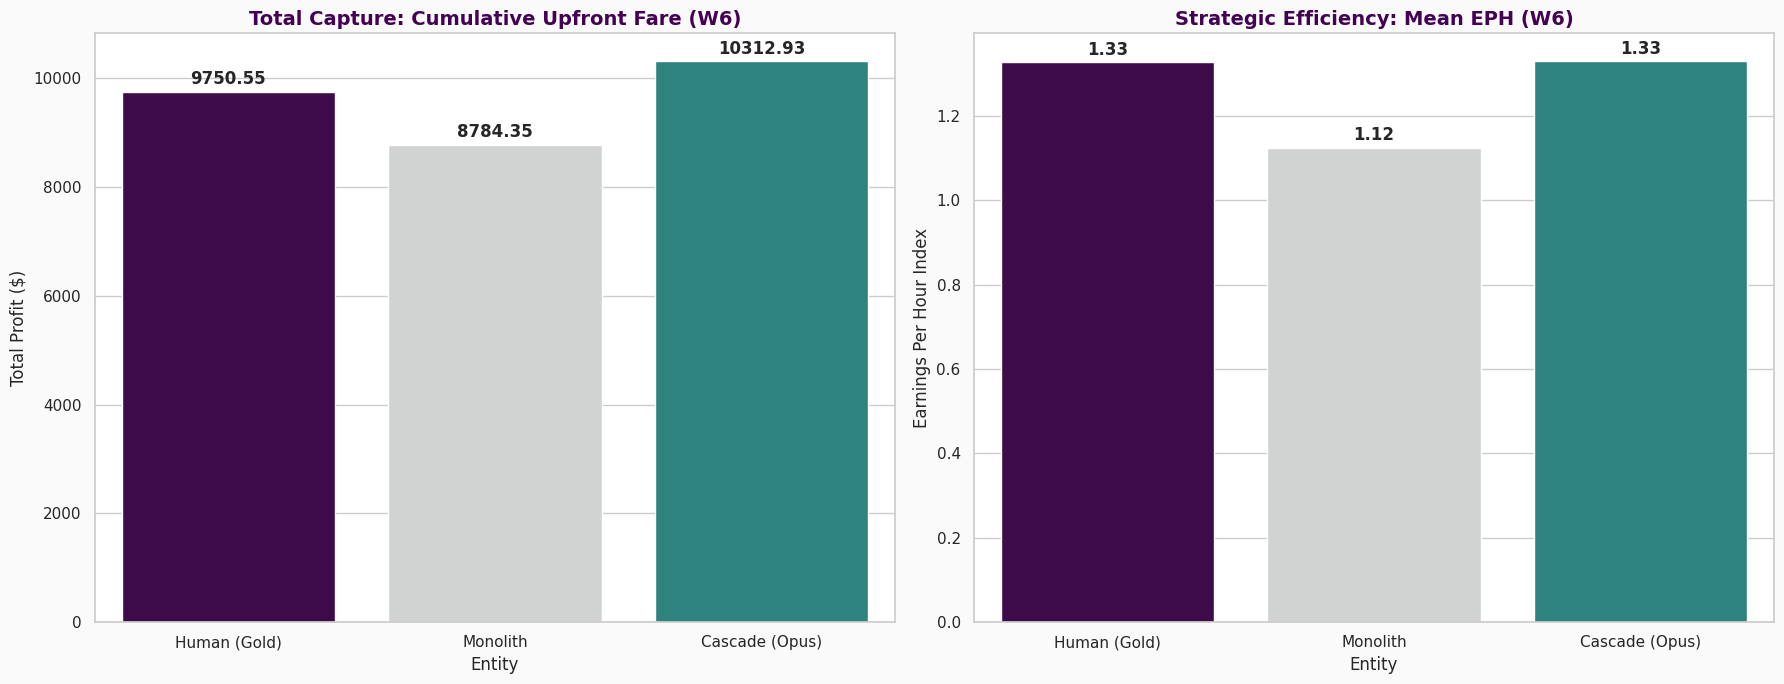
\includegraphics[width=\textwidth]{fig_shadow_mode_results.png} 
    \caption{Shadow Mode Performance Results. The left plot measures total cumulative yield (\$), while the right plot measures strategic efficiency via the mean EPH Index. The Cascade architecture matches the expert’s efficiency while maximizing total value capture.}
    \label{fig:shadow_mode}
\end{figure}

The trial results, illustrated in Figure \ref{fig:shadow_mode}, reveal three critical performance findings:

\begin{itemize}[noitemsep, topsep=3pt]
    \item \textbf{Efficiency Parity:} The \textbf{Cascade (Opus)} model achieved a mean EPH index of \textbf{1.33}, perfectly replicating the Human Agent’s strategic efficiency. This confirms the model successfully learned the high-yield selection criteria required to consistently outperform the market baseline ($1.0$).
    
    \item \textbf{Monolithic Performance Decay:} The monolithic model significantly underperformed, trailing the Human Agent by \textbf{15.7\% in efficiency}. This provides empirical proof that flat architectures are unable to isolate strategic signal from geospatial noise, confirming the negative impact of the "Gravitational Well."
    
    \item \textbf{Volume Surplus (The Machine Advantage):} In a surprising outcome, the Cascade model captured \textbf{5.7\% more total value} than the Human Agent (\$10,312 vs. \$9,750). While maintaining identical efficiency, the machine identified high-yield opportunities that the human agent may have bypassed due to operational fatigue or cognitive load.
\end{itemize}

\noindent \textit{Outcome: The Shadow Mode trial validates the Cognitive Cascade as a high-fidelity behavioral clone. The model demonstrates the ability to match expert strategic efficiency while providing superior consistency in total value capture across a sustained work shift.}

\subsection{Phase 5 Conclusion: Breaking the Static Barrier}
The conclusion of Phase 5 marks the definitive transition from static decision mapping to temporal flow modeling. While the \textit{Cognitive Cascade} successfully isolated the Agent's strategic logic, its performance highlights a fundamental constraint of tabular architectures: \textbf{Snapshot Indifference}. Even when enriched with stateful features, classical \texttt{XGBoost} evaluates offers as isolated events in a vacuum. 

This technical boundary provides the formal validation for the transition to the \textbf{Generative Realm}. To fully deconstruct the \textit{expected\_value\_gamble}---the decision to reject a viable offer based on the probability of a future event---the framework must move beyond independent row analysis. This justifies the scope of Phase 6, where Generative Adversarial Networks (GANs) will synthesize the high-volume data manifolds required to train Recurrent Neural Networks (RNNs). By transforming the market from a sequence of static snapshots into a continuous temporal flow, the Pienza framework moves toward modeling the ``Expert Rhythm,'' where every decision is processed as a dynamic function of the marketplace's heartbeat.




